
\documentclass[]{article}
%\documentclass[journal,10pt,draftclsnofoot,onecolumn]{IEEEtran}
%\usepackage{graphics,multirow,amsmath,amssymb,textcomp,subfigure,multirow,xspace,arydshln,cite}

\usepackage[]{graphicx} 	% para manejar graficos

\usepackage{caption}

\usepackage{enumerate}    % para hacer listas numeradas

\usepackage{amsmath}      	% no se..

\usepackage{amsfonts} 		% no se..

\usepackage{authblk}		% para definir las afiliaciones de cada autor

\usepackage{layout}  		% no se..

\usepackage{biblatex} 		% para manejar la bibliografia / referencias

\usepackage{lipsum}			% para generar texto random

\usepackage{multicol}		% para usar dos columnas

\usepackage{palatino}		% para que la fuente sea palatino

\usepackage[utf8]{inputenc} % para poder usar tildes

%https://tex.stackexchange.com/questions/82993/how-to-change-the-name-of-document-elements-like-figure-contents-bibliogr
\renewcommand{\abstractname}{Abstract} 			% renombro los 'name macros' (mas info en el link de arriba)
\renewcommand{\figurename}{Figure}				% renombro los 'name macros' (mas info en el link de arriba)
\renewcommand{\contentsname}{Table of Contents} % renombro los 'name macros' (mas info en el link de arriba)
\renewcommand{\tablename}{Table}        % renombro los 'name macros' (mas info en el link de arriba)


\usepackage{geometry}
 \geometry{
 a4paper,
 textwidth={17cm},
 textheight={23cm},
 left={2cm},
 top={2.5cm},
 }

\setlength{\columnsep}{1cm} % para que la separacion entre columnas sea de 1 cm

\graphicspath {{imagenes/}}

\defbibheading{bibliography}{\centering} % para que bibtex no imponga su header cuando uso \printbibliography

\addbibresource{bibliografia.bib} % para importar el archivo .bib

\title{\textbf{\LARGE{\textsf{TITÚLO DEL PAPER O INFORME}}}}
 % defino el titulo del Paper

\date{} % lo pongo vacio para que no aparezca abajo del abstract

\usepackage{fancyhdr}

%%%%%%%%%%%%%%%%%%%%%%%%%%%%%%%%%%%%%%%%%%%%%%%%%%%%%%%%%%%%%%%%%%%%%%%%%%%%%%%%%
% http://www-h.eng.cam.ac.uk/help/tpl/textprocessing/multicol_hint.html
\makeatletter 					% esto lo uso para poder definir figuras 
\newenvironment{tablehere}		% esto lo uso para poder definir figuras 
  {\def\@captype{table}}		% esto lo uso para poder definir figuras 
  {}							% esto lo uso para poder definir figuras 
  								% esto lo uso para poder definir figuras 
\newenvironment{figurehere}		% esto lo uso para poder definir figuras 
  {\def\@captype{figure}}		% esto lo uso para poder definir figuras 
  {}							% esto lo uso para poder definir figuras 
\makeatother					% esto lo uso para poder definir figuras 
%%%%%%%%%%%%%%%%%%%%%%%%%%%%%%%%%%%%%%%%%%%%%%%%%%%%%%%%%%%%%%%%%%%%%%%%%%%%%%%%%

%%%%%%%%%%%%%%%%%%%%%%%%%%%%%%%%%%%%%%%%%%%%%%%%%%%%%%%%%%%%%%%%%%%%%%%%%%%%%%%%%
% 							ACA EMPIEZA EL DOCUMENTO                            %
%%%%%%%%%%%%%%%%%%%%%%%%%%%%%%%%%%%%%%%%%%%%%%%%%%%%%%%%%%%%%%%%%%%%%%%%%%%%%%%%%


\begin{document} % empieza el documentoo


\renewcommand{\headrulewidth}{0pt} % para que no haya linea decorativa en el header.


\author[1]{Nombre y Apellido} % defino el autor
\affil[1]{Universidad Nacional de Tres De Febrero, Buenos Aires, Argentina \newline \texttt{email@delautor.com}} % afiliacion del autor


\begin{minipage}[h]{\textwidth} % uso el entorno minipage para que el abstract este en la misma pagina que el titulo
    \maketitle
    \thispagestyle{fancy}
    \fancyhf{}
    \rhead{Fecha de entrega}
    \lhead{Materia/Congreso}
    \cfoot{\thepage}

\end{minipage}


\begin{abstract}

\textit{\lipsum[1]}
\end{abstract}

\begin{multicols}{2}
\section{INTRODUCTION}
\lipsum[2]
\section{RELATED WORKS}
\lipsum[3]
\section{BASIC CONCEPTS AND TERMINOLOGY}
\lipsum[4]
\section{EXPERIMENTAL ARRANGEMENT}
\lipsum[5]
\
For this measurement, valid results can be obtained even with simple equipment.

The instruments used are:
\begin{itemize}
  \item A Tektronix 2049b Osciloscope
  \item A Nike Signal generator
  \item A Ford fiesta
\end{itemize}

\subsection{METHOD 1}
\lipsum[6]
When $\omega$ varies between $0$ and $2 \pi$, figure \ref{fig:circulo} is obtained:

\begin{figurehere}
 \centering
 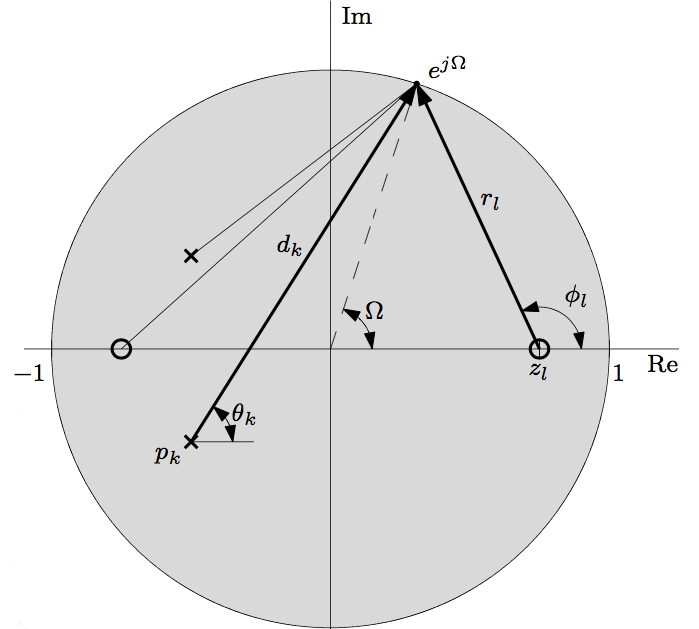
\includegraphics[width=\linewidth]{lathi}
 \captionof{figure}{ poles and los zeros determine $H(z)$}
 \label{fig:circulo}
\end{figurehere}

\subsection{METHOD 2} % SI APLICA
\lipsum[7]
A detailed derivation can be found in \cite{Sh:572} , \cite{Sh:575}.
\subsection{METHOD 3} % SI APLICA
\
\lipsum[8] 
In \cite{webster} se puede ver que:

\begin{equation}
 e^{ \ j  \pi} = -1
 \label{euler}
\end{equation}
This equation \ref{euler} is known as Euler's identity
\section{RESULTS}
Table \ref{Vgs} shows the relation between both variables:
\begin{tablehere}
\begin{center}
\begin{tabular}{|c|c|c|c|}
\hline
$V_{GS}$ [V] & $I_{D}$ [A] & Temperature [$C^{o}$] & $\frac{V_{GS}}{I_D}$ [$\Omega$] \\ 
\hline
col1 & col2 & col3 & col4 \\

col1 & col2 & col3 & col4 \\

col1 & col2 & col3 & col4 \\
\hline
\end{tabular}
\caption{Variation of $\frac{V_{GS}}{I_D}$}
\label{Vgs}
\end{center}
\end{tablehere}
\lipsum[1]


\section{RESULT ANALYSIS}
\lipsum[1]
\section{CONCLUSION}
\lipsum[1]
\section{REFERENCES}
\printbibliography 
\end{multicols}
 


\end{document} 